% siminos/atlas/slice.tex  pdflatex atlas
% $Author$ $Date$


\section{Slice}
% Reduction of continuous symmetry
\label{s:slice}

Suppose your day job is computing invariant solutions of \NSe.
Do you really want to compute the same solution over and over again, for every point on the group orbit?
No, you would like to compute it only once. The rule that picks out that one solution is
called \emph{symmetry reduction}.
Its goal is to replace each group orbit by a
unique point in a lower-dimensional symmetry-\reducedsp\ $\pSRed =
\pS/\Group$, as sketched in \reffig{fig:BeThTraj}.
    \PC{replace the term `symmetry reduction' by a term that does not
    (1) does not imply `reduction' (2) does not conflict with Lie theory
    and gen. relativity meaning of the term
    }

%%%%%%%%%%%%%%%%%%%%%%%%%%%%%%%%%%%%%%%%%%%%%%%%%
% 2011-08-23 Predrag: replaces BeThTraj.pdf from
% dasbuch/book/FigSrc/inkscape/BeThTraj.svg
% 2011-09-09 Predrag: updated
%            continuous.tex overheads, and ChaosBook
\begin{figure}
 \begin{center}
  \setlength{\unitlength}{0.20\textwidth}
  %% \unitlength = units used in the Picture Environment
(a)~~
  \begin{picture}(1,1.07471658)%
    \put(0,0){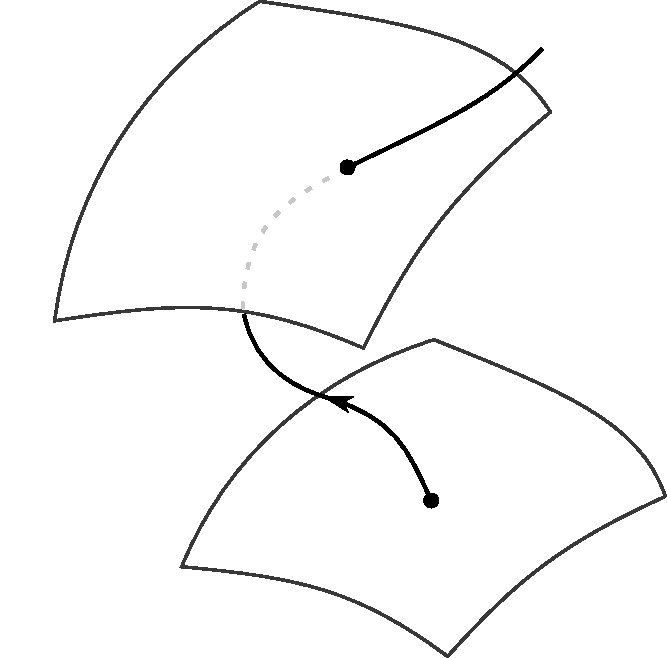
\includegraphics[width=\unitlength]{BeThTrajTeX}}%
    \put(0.28879298,1.02196543){\color[rgb]{0,0,0}\rotatebox{-22.37140782}{\makebox(0,0)[lb]{\smash{$\pS_{\ssp(\zeit)}$}}}}%
    \put(0.55566402,0.45078735){\color[rgb]{0,0,0}\rotatebox{-16.6673442}{\makebox(0,0)[lb]{\smash{$\pS_{\ssp(0)}$}}}}%
    \put(0.63028127,0.18433597){\color[rgb]{0,0,0}\rotatebox{0.03136739}{\makebox(0,0)[lb]{\smash{$\ssp(0)$}}}}%
    \put(0.46253394,0.70182304){\color[rgb]{0,0,0}\rotatebox{0.03136739}{\makebox(0,0)[lb]{\smash{$\ssp(\zeit)$}}}}%
    \put(0.03852492,0.09250899){\color[rgb]{0,0,0}\rotatebox{0.11031334}{\makebox(0,0)[lb]{\smash{$\pS$}}}}%
  \end{picture}%
~~(b)
  \begin{picture}(1,1.07315413)%
    \put(0,0){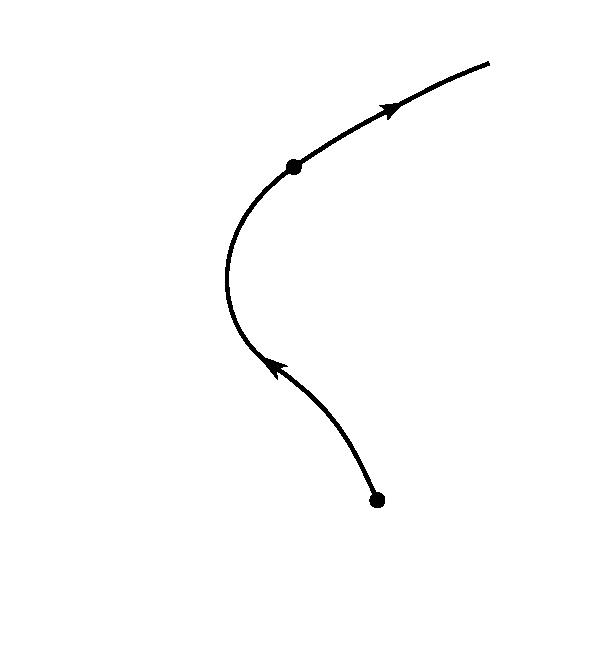
\includegraphics[width=\unitlength]{BeThRedTeX}}%
    \put(0.19912369,0.17144733){\color[rgb]{0,0,0}\rotatebox{0.11031334}{\makebox(0,0)[lb]{\smash{$\pSRed$}}}}%
    \put(0.63028127,0.18433598){\color[rgb]{0,0,0}\rotatebox{0.03136739}{\makebox(0,0)[lb]{\smash{$\sspRed(0)$}}}}%
    \put(0.46253394,0.70182305){\color[rgb]{0,0,0}\rotatebox{0.03136739}{\makebox(0,0)[lb]{\smash{$\sspRed(\zeit)$}}}}%
  \end{picture}%
 \end{center}
% (a) 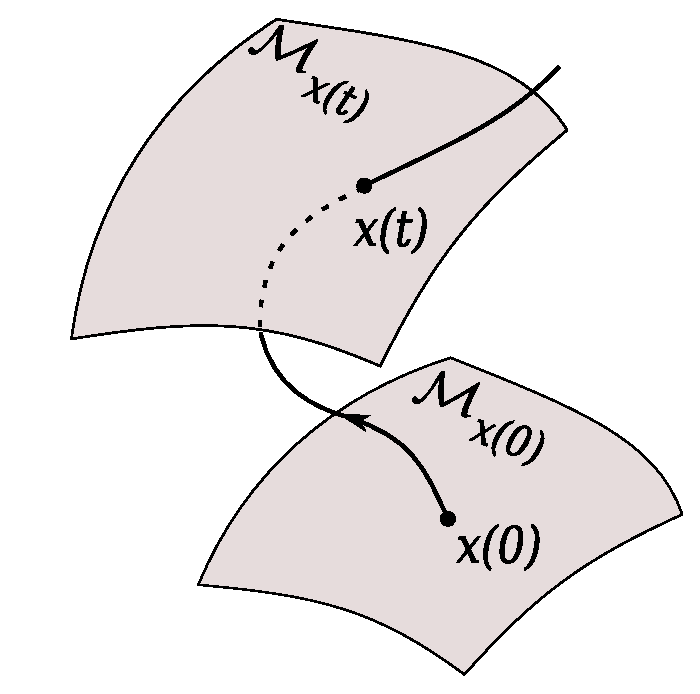
\includegraphics[width=0.45\textwidth]{BeThTraj}
  \caption{\label{fig:BeThTraj}
(a)
The group orbit $\pS_{\ssp(0)}$ of \statesp\ point $\ssp(0)$, and the
group orbit $\pS_{\ssp(\zeit)}$ reached by the trajectory $\ssp(\zeit)$ time $t$
later.
(b)
Symmetry reduction $\pS \to \pSRed$ replaces $\pS_{\ssp}\subset\pS$ by a
single point $\sspRed \in \pSRed$.
  }
\end{figure}
%%%%%%%%%%%%%%%%%%%%%%%%%%%%%%%%%%%%%%%%%%%%%%%%%%

What is a smart way to go about it? Intuition gained from pipe flow (see
\reffig{fig:A27-pipeSymms}), will again prove helpful. A turbulent flow
exhibits a myriad of unstable structures, all travelling down the pipe,
each with its own {\phaseVel}. The
\mslices\rf{rowley_reconstruction_2000,BeTh04,SiCvi10,FrCv11} that we now
describe tells you how to pull each solution back into a {\em fixed}
frame, the \slice, and there compare it to your repertoire of precomputed
solutions, the \template s $\{\slicep{}^{(j)}\}$, by a very geometrical
principle of the closest distance to each. What follows is very much like
the construction of sections of \refsect{s:cut}; due to the linear action
of the symmetry group, slicing is easier than sectioning, but is wholly
unfamiliar - that is why we warmed up by reviewing the Poincar\'e
sections. We now offer a pictorial tour of this hitherto uncharted
territory, save for the one bold incursion\rf{ACHKW11}.

First, one picks a \template\ $\slicep$ and uses the freedom to choose a moving frame
(\reffig{fig:slice}) to shift and rotate $\slicep$ until it overlies, as
well as possible, the state $\ssp$, by minimizing the
distance
\beq
\Norm{\ssp - \LieEl(\gSpace)\,\slicep}
\, .
\ee{minDistance}
The entire group orbit of $\ssp$ is then replaced by the closest match to
the template pattern, given by $\sspRed=\LieEl^{-1}\ssp$. The
symmetry-\reducedsp\ $\pSRed$ is comprised of such closest matches
$\sspRed$, a point for each full \statesp\ group orbit; the hat on
$\sspRed$ indicates the unique point on the group orbit of $\ssp$ closest
to the \template\ \slicep.

%%%%%%%%%%%%%%%%%%%%%%%%%%%%%%%%%%%%%%%%%%%%%%%%%%%%%%%%%%%%%%%%%%%%%
\begin{figure}
	\begin{center}
  	\setlength{\unitlength}{0.25\textwidth}
  	\begin{picture}(1,0.62007592)%
    	\put(0,0){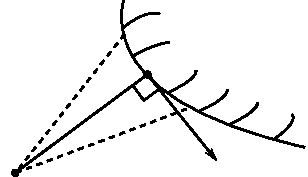
\includegraphics[width=\unitlength]{A28extremum2}}%
    	\put(0.8274739,0.27313042){\color[rgb]{0,0,0}\makebox(0,0)[lb]{\smash{$\LieEl\,\ssp$}}}%
    	\put(0.71822871,0.05712263){\color[rgb]{0,0,0}\makebox(0,0)[lb]{\smash{$\sliceTan{}$}}}%
    	\put(-0.00055527,0.03229441){\color[rgb]{0,0,0}\makebox(0,0)[lb]{\smash{$\slicep$}}}%
    	\put(0.50966967,0.33520145){\color[rgb]{0,0,0}\makebox(0,0)[lb]{\smash{$\sspRed$}}}%
  	\end{picture}
  \end{center}
  \caption{\label{fig:A28extremum}
  Extremal condition \refeq{PCsectQ0} for the point $\sspRed$ on the
  $\ssp$ group orbit that is nearest to the \template\ $\slicep$.
  }
\end{figure}
%%%%%%%%%%%%%%%%%%%%%%%%%%%%%%%%%%%%%%%%%%%%%%%%%%%%%%%%%%%%%%%%%%%%%


The minimal distance satisfies
the extremum condition (\reffig{fig:A28extremum})
\[
\frac{\partial}{\partial \gSpace} \Norm{\ssp - \LieEl(\gSpace)\,\slicep}^2
   =
2\, \braket{\sspRed - \slicep}{\sliceTan{}}
   = 0
        \,,\quad
\sliceTan{} = \Lg \slicep
\,.
\]
$\Norm{\LieEl(\gSpace)\slicep}$ is a constant, the group tangent vector
$\sliceTan{}$ evaluated at $\slicep$ \refeq{eq:tang} is normal to
$\slicep$, and the term $\braket{\slicep}{\Lg \,\slicep}$ vanishes ($\Lg$
is antisymmetric). Therefore  $\sspRed$, the point on the group orbit
of $\ssp$ that lands in the \slice, satisfies the \emph{\slice\ condition} 
\DB{04-13-2012}{\Lg is not defined anywhere up till now}

\beq
\braket{\sspRed}{\sliceTan{}} = 0
    \,.
\ee{PCsectQ0}
The \slice\ so defined is thus a $(d\!-\!N)$\dmn\ hyperplane normal to
the $N$ group tangents evaluated at the \slicep, as sketched in
\reffig{fig:slice}. This is a highly idealized sketch: A group orbit is a
$N$\dmn\ manifold and even for $\SOn{2}$ it is usually only
topologically a circle, and can intersect a hyperplane any number of
times  (see \reffigs{fig:sliceimage}{fig:chartBord}).

\DBedit{As $\ssp$ varies in time, the {\template}
$\slicep$ tracks the motion using the slice condition \refeq{PCsectQ0} to
minimize $\Norm{\ssp(\zeit)-\LieEl(\phi(\zeit))\slicep}$, and the
full-space trajectory $\ssp(\zeit)$ is thus rotated into the
{\reducedsp} $\pSRed$ by appropriate
time varying \emph{moving frame} angles $\{\gSpace(\zeit)\}$, as depicted
in \reffig{fig:slice}\,{(a)}. One can write the equations for the
flow in the \reducedsp\, $\dot{\sspRed} = \velRed(\sspRed)$, which confine the motion to the
\slice (i.e., $\sspRed(\zeit) \in \pSRed$), as
\bea
\velRed(\sspRed) &=& \vel(\sspRed)
     \,-\, \dot{\gSpace}(\sspRed) \, \groupTan(\sspRed)
\label{EqMotMFrame}\\
\dot{\gSpace}(\sspRed) &=& \braket{\vel(\sspRed)}{\sliceTan{}}
                       /\braket{\groupTan(\sspRed)}{\sliceTan{}}
\,.
\label{reconstrEq}
\eea
The velocity in the full \statesp\ $\vel$ is then the sum of $\velRed$,
the velocity component in the \slice, and $\dot{\gSpace}\,\groupTan$, the
velocity component within the group tangent space. The $\dot{\gSpace}$
equation is called the {\em reconstruction equation}, as its integral
keeps track of the group shift in the full \statesp.}

The {\template} $\slicep$ should be a generic \statesp\ point in the
sense that its group orbit has the full $N$ dimensions of the group
\Group. The set of the group orbit points \emph{closest} to the
\template\ \slicep\ forms a neighborhood of \slicep\ in which each group
orbit intersects the hyperplane \emph{only once}.
A \slice\ hyperplane captures neighboring group orbits until,
for a point $\sspRSing$ not so close to the \template, the group tangent vector
lies in the \slice. The group orbits for such points are grazed tangentially rather than sliced
transversally, much like what happens at the \poincBord\
\refeq{eq:sspRSing} for evolution in time. This is
also a linear condition, and it defines the {\sliceBord} ${\cal S}$ \DB{2012-04-13}{Are we using $\cal{S}$ for both section and slice borders?}, a
hyperplane in which both points $\sspRSing$ and their group tangents
$\groupTan(\sspRSing)$ lie in the {\slice},\rf{FrCv11}
\beq
\braket{\sspRSing}{\sliceTan{}} \,=\, 0
      \mbox{ and }
\braket{\groupTan(\sspRSing)}{\sliceTan{}} \,=\, 0
\,.
\label{sliceSingl0}
\eeq
We shall refer to this neighborhood of a \template\ \slicep\ bounded by its
{\chartBord} and the ridges with other such linear neighborhoods as a
\emph{chart} $\pSRed_{\slicep} \supset \pS/\Group$, and to
\refeq{PCsectQ0} as the \DBedit{\emph{border conditions}}.\DB{2012-04-13}{\refeq{sliceSingl0} is more restrictive than \refeq{PCsectQ0}. It also defines the slice border rather than a slice.}

%%%%%%%%%%%%%%%%%%%%%%%%%%%%%%%%%%%%%%%%%%%%%%%%%%%%%%%%%%%%%%%%
%% slice.*, inflectHype.*: see dasbuch/book/FigSrc/inkscape/00ReadMe.txt
%% rpo.* hand-drawn in dasbuch/book/FigSrc/xfig/rpo.fig
%% xfig exported -> FigSrc/inkscape/rpo.fig
%% inkscape exported -> rpo.eps + LaTeX, hand edited in the macros
%% Predrag 2011-08-27 replaced rpo.pdf by rpoSlice.pdf
%% remember to insert rpoSlice.pdf into ChaosBook

 \begin{figure}
 \begin{center}
  \setlength{\unitlength}{0.30\textwidth}
  %% \unitlength = units used in the Picture Environment
(a)
  \begin{picture}(1,0.87085079)%
    \put(0,0){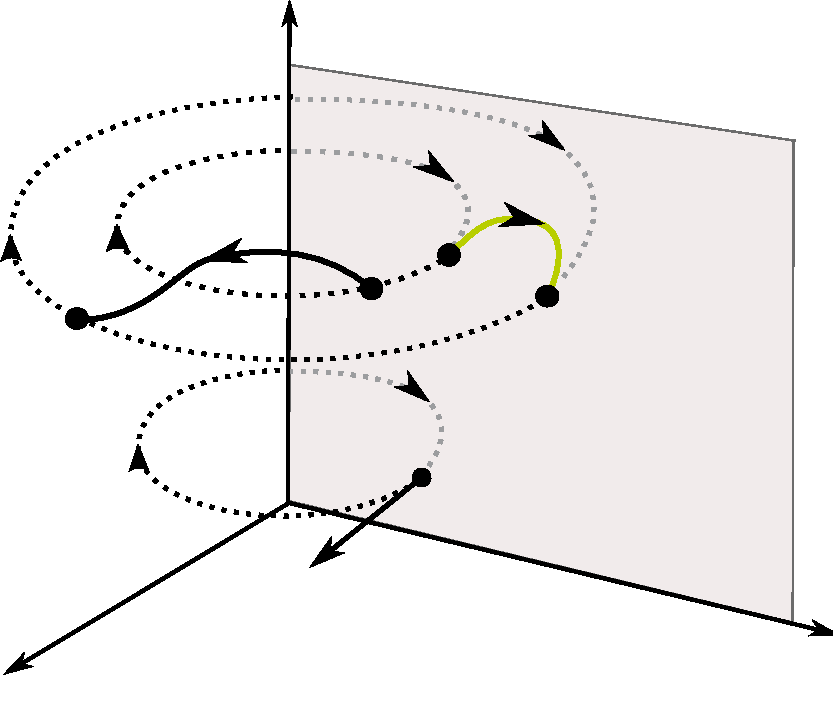
\includegraphics[width=\unitlength]{slice}}%
    \put(0.82835155,0.19007659){\color[rgb]{0,0,0}\rotatebox{-14.84025424}{\makebox(0,0)[lb]{\smash{$\pSRed$}}}}%
    \put(0.06577338,0.28688228){\color[rgb]{0,0,0}\rotatebox{0.0313674}{\makebox(0,0)[lb]{\smash{$\LieEl\,\slicep$}}}}%
    \put(0.53023327,0.26593335){\color[rgb]{0,0,0}\rotatebox{0.0313674}{\makebox(0,0)[lb]{\smash{$\slicep$}}}}%
    \put(0.4284954,0.179285){\color[rgb]{0,0,0}\rotatebox{0.0313674}{\makebox(0,0)[lb]{\smash{$\sliceTan{}$}}}}%
    \put(0.00798985,0.42305068){\color[rgb]{0,0,0}\rotatebox{0.0313674}{\makebox(0,0)[lb]{\smash{$\ssp(\zeit)$}}}}%
    \put(0.65766235,0.45412105){\color[rgb]{0,0,0}\rotatebox{0.0313674}{\makebox(0,0)[lb]{\smash{$\sspRed(\zeit)$}}}}%
    \put(0.06916446,0.74280851){\color[rgb]{0,0,0}\rotatebox{0.0313674}{\makebox(0,0)[lb]{\smash{$\LieEl\,\ssp(\zeit)$}}}}%
  \end{picture}%
\\ %~~~
(b)
  \begin{picture}(1,0.87085079)%
    \put(0,0){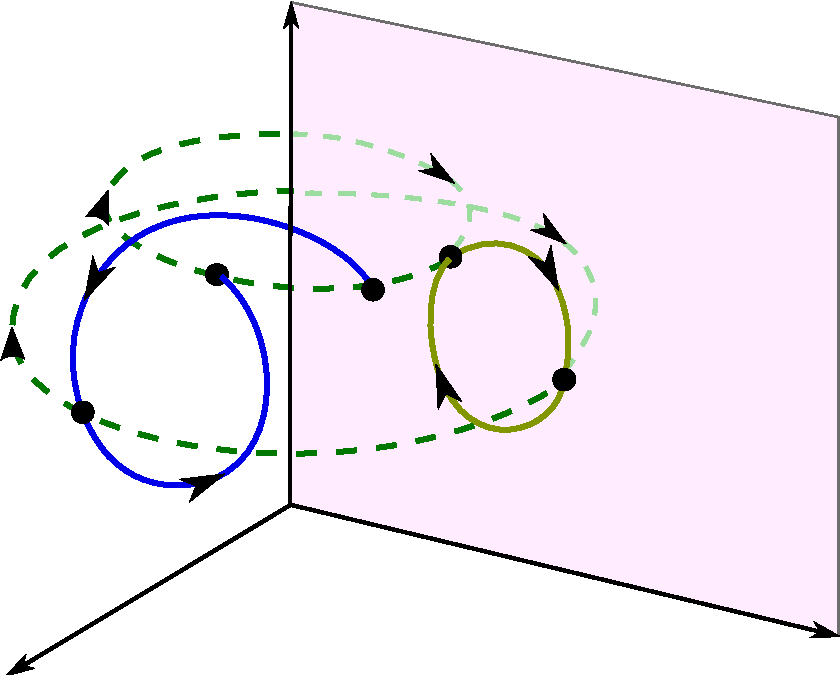
\includegraphics[width=\unitlength]{rpoSlice}}%
    \put(0.82835153,0.19007656){\color[rgb]{0,0,0}\rotatebox{-14.84025432}{\makebox(0,0)[lb]{$\pSRed$}}}%
    \put(0.40925459,0.45713857){\color[rgb]{0,0,0}\rotatebox{0.0313674}{\makebox(0,0)[lb]{\smash{$\ssp(0)$}}}}%
    \put(0.71354118,0.39765314){\color[rgb]{0,0,0}\rotatebox{0.0313674}{\makebox(0,0)[lb]{\smash{$\sspRed(\zeit)$}}}}%
    \put(0.13171187,0.38813817){\color[rgb]{0,0,0}\rotatebox{0.0313674}{\makebox(0,0)[lb]{\smash{$\LieEl(\zeit)$}}}}%
    \put(0.02168739,0.31359574){\color[rgb]{0,0,0}\rotatebox{0.0313674}{\makebox(0,0)[lb]{\smash{$\ssp(\zeit)$}}}}%
    \put(0.15576193,0.48769256){\color[rgb]{0,0,0}\rotatebox{0.0313674}{\makebox(0,0)[lb]{\smash{$\ssp(\period{})$}}}}%
    \put(0.54113911,0.50476963){\color[rgb]{0,0,0}\rotatebox{0.0313674}{\makebox(0,0)[lb]{\smash{$\sspRed(0)$}}}}%
  \end{picture}%
 \end{center}
 \caption{
The \mslices, a \statesp\ visualization:
(a)
\Slice\ $\pSRed \supset \pS/\Group$ lies in the $(d\!-\!N)$\dmn\
hyperplane \refeq{PCsectQ0} normal to $\sliceTan{j}$, which
span the $N$\dmn\ space tangent to the group orbit $\LieEl\,\slicep$
(dotted line) evaluated at the {\template} point $\slicep$. The
hyperplane intersects {all} full \statesp\ group orbits (green
dashes).  The full \statesp\
trajectory $\ssp(\zeit)$ (blue) and the \reducedsp\ trajectory
$\sspRed(\zeit)$ (green) are equivalent up to a `moving frame' rotation
$\ssp(\zeit)=\LieEl(\zeit)\,\sspRed(\zeit)$, where $\LieEl(\zeit)$ is a
shorthand for $\LieEl(\gSpace(\zeit))$.
(b)
In the full \statesp\ a \rpo\ $\ssp(0) \to \ssp(\zeit) \to
\ssp(\period{})$ returns to the group orbit of $\ssp(0)$ after time
$\period{}$ and a rotation by $\LieEl$,  $\ssp(0)=\LieEl \, \ssp
(\period{})$. A generic \rpo\ quasi-\-periodically fills out what is
topologically a torus (\reffig{fig:CLf01group}\,(b)). In the \slice\ $\pSRed$
the symmetry-reduced trajectory is periodic, $\sspRed(0) =
\sspRed(\period{})$.
 }\label{fig:slice}
 \end{figure}

\DBedit{The \mslices\ is akin to (but distinct from) cutting across trajectories by
means of sections. Both methods reduce continuous symmetries: Poincar\'e
sections cut the spaghetti of the continuous-time trajectories, slices cut the layers of the onion of group-orbits. Both are triggered by certain condition: oriented
piercing of the section, or the slice condition. Just as a Poincar\'e
section goes bad, a slice goes bad the moment transversality is lost.  A \PoincSec\ reduces a continuous time trajectory to a sequence of
points. A \slice, however, is emphatically \emph{not} a \PoincSec; it
replaces a trajectory by a symmetry-reduced trajectory.} % Minor rewording
